\documentclass[tikz,border=10pt]{standalone}
\usetikzlibrary{arrows.meta, positioning}
\begin{document}
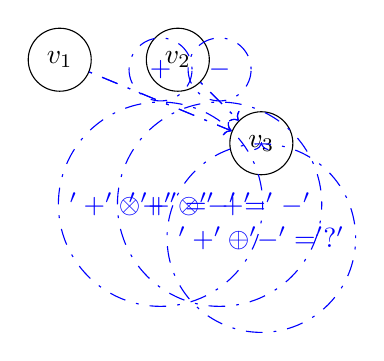
\begin{tikzpicture}[
node distance=1.5cm and 2cm,
every node/.style={draw, circle, minimum size=8mm},
arrow style/.style={blue, dash pattern=on 1pt off 4pt on 6pt off 4pt}
]

% Nodes
\node(v1){$v_1$};
\node(v2)[right of=v1]{$v_2$};
\node(v3)[below right of=v2]{$v_3$};

% Arrows
\draw[->, arrow style] (v1) -- node[above]{$+$} (v3);
\draw[->, arrow style] (v2) -- node[above]{$-$} (v3);

\draw[dashed, -> , arrow style] (v1) -- node[below]{$'+' \otimes '+' = '+'$} (v3);
\draw[dashed, -> , arrow style] (v2) -- node[below]{$'+' \otimes '-' = '-'$} (v3);
\draw[dashed, -> , arrow style] (v3) -- node[below]{$'+' \oplus '-' = '?'$} (v3);

\end{tikzpicture}
\end{document}